\documentclass[a4paper,11pt]{article}
\usepackage{amsmath,amsthm,amsfonts,amssymb,amscd,amstext,vmargin,graphics,graphicx,tabularx,multicol} \usepackage[french]{babel}
\usepackage[utf8]{inputenc}  
\usepackage[T1]{fontenc} 
\usepackage[T1]{fontenc}
\usepackage{amsmath,amssymb}
\usepackage{pstricks-add,tikz,tkz-tab,variations}
\usepackage[autolanguage,np]{numprint} 

\setmarginsrb{1.5cm}{0.5cm}{1cm}{0.5cm}{0cm}{0cm}{0cm}{0cm} %Gauche, haut, droite, haut
\newcounter{numexo}
\newcommand{\exo}[1]{\stepcounter{numexo}\noindent{\bf Exercice~\thenumexo} : \marginpar{\hfill /#1}}
\reversemarginpar


\newcounter{enumtabi}
\newcounter{enumtaba}
\newcommand{\q}{\stepcounter{enumtabi} \theenumtabi.  }
\newcommand{\qa}{\stepcounter{enumtaba} (\alph{enumtaba}) }
\newcommand{\initq}{\setcounter{enumtabi}{0}}
\newcommand{\initqa}{\setcounter{enumtaba}{0}}

\newcommand{\be}{\begin{enumerate}}
\newcommand{\ee}{\end{enumerate}}
\newcommand{\bi}{\begin{itemize}}
\newcommand{\ei}{\end{itemize}}
\newcommand{\bp}{\begin{pspicture*}}
\newcommand{\ep}{\end{pspicture*}}
\newcommand{\bt}{\begin{tabular}}
\newcommand{\et}{\end{tabular}}
\renewcommand{\tabularxcolumn}[1]{>{\centering}m{#1}} %(colonne m{} centrée, au lieu de p par défault) 
\newcommand{\tnl}{\tabularnewline}

\newcommand{\trait}{\noindent \rule{\linewidth}{0.2mm}}
\newcommand{\hs}[1]{\hspace{#1}}
\newcommand{\vs}[1]{\vspace{#1}}

\newcommand{\N}{\mathbb{N}}
\newcommand{\Z}{\mathbb{Z}}
\newcommand{\R}{\mathbb{R}}
\newcommand{\C}{\mathbb{C}}
\newcommand{\Dcal}{\mathcal{D}}
\newcommand{\Ccal}{\mathcal{C}}
\newcommand{\mc}{\mathcal}

\newcommand{\vect}[1]{\overrightarrow{#1}}
\newcommand{\ds}{\displaystyle}
\newcommand{\eq}{\quad \Leftrightarrow \quad}
\newcommand{\vecti}{\vec{\imath}}
\newcommand{\vectj}{\vec{\jmath}}
\newcommand{\Oij}{(O;\vec{\imath}, \vec{\jmath})}
\newcommand{\OIJ}{(O;I,J)}

\newcommand{\bmul}[1]{\begin{multicols}{#1}}
\newcommand{\emul}{\end{multicols}}


\newcommand{\reponse}[1][1]{%
\multido{}{#1}{\makebox[\linewidth]{\rule[0pt]{0pt}{20pt}\dotfill}
}}

\newcommand{\titre}[5] 
% #1: titre #2: haut gauche #3: bas gauche #4: haut droite #5: bas droite
{
\noindent #2 \hfill #4 \\
#3 \hfill #5

\vspace{-1.6cm}

\begin{center}\rule{6cm}{0.5mm}\end{center}
\vspace{0.2cm}
\begin{center}{\large{\textbf{#1}}}\end{center}
\begin{center}\rule{6cm}{0.5mm}\end{center}
}



\begin{document}
\pagestyle{empty}
\titre{Contrôle : Nombres relatifs, périmètres et aires}{Nom :}{Prénom :}{Classe}{Date}


\exo{2.5}  Calculer les expressions  suivantes :

\bmul{2}
$V= +10 - (-32) - (+7) + (-9)$

\columnbreak
$I= - 7,5 - (18 - 7,3) - (2 - 14,5)$
\emul




\exo{3}

\initq 
\noindent \q Placer sur une droite graduée les points A, B et C d'abscisses respectives 2,3 ; -3,7 et -0,7.\\
\q Calculer les distances AC et BC.\\
\q Que peut-on dire du point C ? (Justifier)\\


\exo{6} 

\bmul{2}
Des enfants lancent 4 fléchettes sur la cible représentée ci-contre.\\
On obtient :\\
\bi
\item 5 points pour un tir dans le rouge,
\item 2 points pour un tir dans le vert,
\item -1 point pour un tir dans le bleu,
\item -10 points si on rate la cible.
\ei

\columnbreak

\begin{center}
 
\includegraphics[scale=1]{cible.eps}
 \end{center} 
\emul

Voici les résultats des 4 compétiteurs :\\
\bmul{2}
\noindent Anaïs : rouge, vert, vert, raté\\
David : rouge, vert, bleu, raté

\columnbreak

\noindent Eva : rouge, raté, raté, rouge\\
Sacha : vert, vert, bleu, raté

\emul

\initq
\q 
\qa Écrire l'expression qui permet de calculer le score de chaque enfant, puis calculer ce score.\\

\qa Ranger ces scores par ordre croissant.\\

\q Un enfant a obtenu le score de -31. Quels sont ses 4 lancers ?\\



\exo{3} Calculer le périmètre des figures suivantes :\\


\bmul{3}

\begin{flushleft}
\initqa \qa \includegraphics[scale=0.4]{perim1.eps} 
\end{flushleft}

\columnbreak

\begin{flushleft}
\qa \includegraphics[scale=0.4]{perm2.eps} 
\end{flushleft}

\columnbreak

\begin{flushleft}
\qa \includegraphics[scale=0.4]{perim3.eps} 
\end{flushleft}

\emul


\exo{4}\\

\initq \q Calculer l'aire d'un disque de diamètre 20m.\\

\q Un rectangle a une longueur de 2,5 cm et une aire de 12.5 $cm^{2}$. Calculer sa largeur.\\

\newpage

\q Le rectangle et le carré ci-dessous ont le même périmètre.
Calculer l'aire du carré.

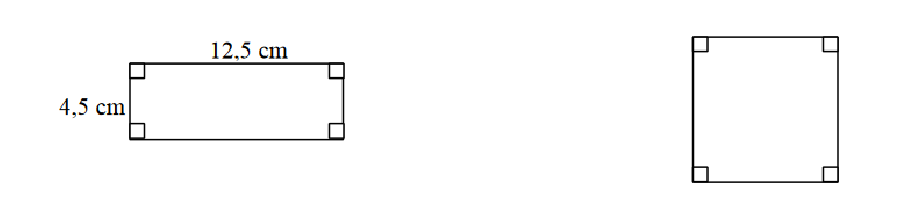
\includegraphics[scale=1]{aires3.eps} \\




\exo{1.5} 

\begin{center}
\includegraphics[scale=0.9]{aires1.eps} 
\end{center}


\noindent \initq \q Calculer l'aire, en $cm^{2}$ du polygone ci-dessus.\\
\q Exprimer l'aire du polygone en $dm^{2}$ .\\





\exo{} BONUS\\

Je suis un rectangle dont les côtés mesurent un nombre entier de centimètres. Mon aire est égale a 120 $cm^{2}$ et mon périmètre est égal à 52 cm. \\
Quelles sont mes dimensions ?\\



\end{document}
